\documentclass[a4paper,12pt]{report}
\usepackage[utf8]{inputenc}
\usepackage{graphicx}
\usepackage{hyperref}
\usepackage{amsmath}
\usepackage{fancyhdr}
\usepackage{geometry}
\geometry{margin=1in}
\usepackage{listings}
\usepackage{tocbibind}

% Header and footer settings
\pagestyle{fancy}
\fancyhf{}
\fancyhead[L]{Synth Net}
\fancyhead[R]{\leftmark}
\fancyfoot[C]{\thepage}

\title{Synth Net: I2C Communication in Microcontrollers}
\author{Reto Ramirez}
\date{May 2024}
\institution{University of Houston}

\begin{document}

% 1. Cover Page (Portada)
\maketitle

% 2. Table of Contents (Índice)
\tableofcontents
\newpage

% 3. Executive Summary (Resumen Ejecutivo)
\chapter*{Executive Summary}
\addcontentsline{toc}{chapter}{Executive Summary}
Synth Net is a project that integrates four microcontrollers (two ESP32s, an Arduino Uno, and an Arduino Mega) connected via I2C communication on a single breadboard. The primary goal of Synth Net is to achieve efficient bidirectional communication between these devices, overcoming the limitations of existing libraries. Each microcontroller has a specific role: one ESP32 acts as the master, managing the overall communication, the Arduino Mega displays collected information in a custom interface, another ESP32 retrieves weather data through an API, and the Arduino Uno gathers environmental data using sensor modules. This project not only posed significant technical challenges but also served as a personal source of motivation during a difficult period of health.
\newpage

% 4. Introduction (Introducción)
\chapter{Introduction}
After enduring a challenging year with health issues related to cancer, I felt the need to engage in a project that would present a fun and stimulating challenge while helping me regain a sense of purpose. Synth Net was born out of this need, serving as both an exploration into I2C communication across multiple microcontrollers and a platform to showcase my work in my first science fair.

The decision to work with I2C communication was intentional, given its complexity. Managing a bus with multiple devices and writing approximately 1,500 lines of code introduced unique challenges, particularly with library compatibility and conflicts. However, overcoming these obstacles allowed me to dive deeper into advanced microcontroller concepts and serial communication techniques.

The core objective of Synth Net was to establish efficient bidirectional communication within a system composed of four microcontrollers, using libraries that did not natively support this functionality. Custom functions were developed to enable smooth integration and coordination between the components.
\section{Motivation}
Explanation of the importance of the addressed challenge, for example, the need for low-cost environmental monitoring systems.

% 5. Project Objectives (Objetivos del Proyecto)
\section{Objectives}
\subsection{General Objective}
The primary goal of Synth Net is to develop an integrated system that enables efficient bidirectional communication between four microcontrollers—two ESP32 units, an Arduino Uno, and an Arduino Mega—using the I2C protocol. This system overcomes the inherent limitations of standard libraries by implementing custom functions tailored to support complex communication scenarios across multiple devices. The project seeks to optimize data exchange, processing, and display, creating a cohesive network where each microcontroller performs distinct, yet interdependent, roles.

\subsection{Specific Objectives}
\begin{itemize}
    \item Configure two ESP32 microcontrollers, an Arduino Uno, and an Arduino Mega on a shared breadboard, establishing a robust I2C communication architecture.
    \item Assign distinct roles to each microcontroller: one ESP32 will act as the master controlling the communication flow, the Arduino Mega will handle data visualization, the second ESP32 will retrieve real-time weather data via an API, and the Arduino Uno will gather environmental data through attached sensors.
    \item Develop custom I2C communication functions that facilitate seamless bidirectional data transmission between the devices, effectively bypassing the limitations imposed by standard libraries.
    \item Design and implement a custom graphical interface on the Arduino Mega that organizes and displays the collected data in a clear and user-friendly manner.
    \item Conduct comprehensive testing to ensure the system’s stability, reliability, and seamless integration of all components, addressing potential hardware and software challenges.
\end{itemize}

\newpage

% 6. Theoretical Framework (Marco Teórico)
\chapter{Theoretical Framework}
This section presents the key concepts used in the Synth Net project, such as microcontrollers, the I2C communication protocol, and climate API integration.

\section{Microcontrollers}

ESP32: A high-performance microcontroller with built-in Wi-Fi and Bluetooth capabilities, the ESP32 is well-suited for applications that require wireless connectivity. Its powerful dual-core processor and abundant I/O options make it an ideal choice for managing complex tasks like coordinating a network of multiple devices.
Arduino Uno and Mega: These popular microcontrollers, based on the ATmega328P (Uno) and ATmega2560 (Mega), are widely used due to their simplicity, large community support, and compatibility with a variety of sensors and modules. The Mega, with its increased memory and input/output pins, is ideal for handling more intensive tasks such as graphical data display.

\section{I2C Communication}
The I2C (Inter-Integrated Circuit) protocol is a synchronous serial communication standard that allows multiple devices to communicate with one another using just two lines: SDA (data) and SCL (clock). Designed for efficient and reliable data transfer between microcontrollers and peripherals, I2C operates in a master-slave configuration. In Synth Net, the ESP32 serves as the master, directing communication between the microcontrollers and ensuring that data is transmitted and received without conflict, even in a highly concurrent system.

\section{Climate APIs}
The integration of external APIs, such as OpenWeather, enables the system to access real-time weather information. Using HTTP requests, the ESP32 retrieves JSON-formatted data, which is then parsed and optimized for minimal memory usage. Efficient serialization and deserialization are critical to ensure that only essential data is transmitted over the I2C bus, maintaining optimal system performance while minimizing overhead.

\newpage

% 7. System Description (Descripción del Sistema Synth Net)
\chapter{Synth Net System Description}
\section{General Architecture}
Synth Net consists of four microcontrollers interconnected on a single breadboard, utilizing the I2C protocol for communication. The architecture is designed in a master-slave configuration, where one ESP32 functions as the master and coordinates communication between the other devices. This architecture enables seamless data exchange and integration between the microcontrollers, each performing distinct tasks critical to the overall system functionality.

(A block diagram illustrating the interconnection between the microcontrollers and their specific roles will be inserted here.)
\section{Roles of Each Component}
\subsection{ESP32 Master}
Functions and Responsibilities:
Manages I2C communication between all devices, acting as the central coordinator.
Hosts a local web server that provides an alternative method for data input, allowing users to interact with the system remotely.
Handles requests and responses from the slave devices, ensuring smooth data flow and execution of tasks.
\subsection{Arduino Mega}
Functions and Responsibilities:
Responsible for rendering graphical elements such as logos and managing variables for display.
Displays a custom interface built in C, which presents the collected data in a clear, organized format. The interface facilitates real-time monitoring of system performance and environmental conditions.

\subsection{ESP32 with Climate API}
Data Integration and Retrieval:
Connects to the internet via Wi-Fi to retrieve real-time weather data through the OpenWeather API.
Parses the received JSON data and optimizes it by reducing the number of bytes, minimizing memory and storage usage, and ensuring efficient data transfer over the I2C bus.
\subsection{Arduino Uno}
Environmental Data Collection:
Gathers environmental data using connected sensor modules, such as temperature and humidity sensors.
Sends the collected data to the ESP32 master for further processing and visualization on the Arduino Mega.

\section{Connections and Communication}
The communication between microcontrollers is established using the I2C protocol, with each device connected to the SDA (data) and SCL (clock) lines. These two lines facilitate bidirectional data transfer, allowing the ESP32 master to coordinate the flow of information between the microcontrollers. Custom functions were developed to optimize communication efficiency and resolve potential conflicts between libraries, ensuring stable operation under varying workloads.
\newpage

% 8. Materials and Components Used (Materiales y Componentes Utilizados)
\chapter{Materials and Components Used}

    
    \chapter{Materials and Components Used}
    Complete list of hardware:
    
    \begin{itemize}
        \item \textbf{2 x ESP32}: High-performance microcontroller with Wi-Fi and Bluetooth capabilities.
        \item \textbf{1 x Arduino Uno}: Microcontroller based on ATmega328P.
        \item \textbf{1 x Arduino Mega}: Microcontroller with extended memory and I/O pins based on ATmega2560.
        \item \textbf{Breadboard}: Sufficient size to host all components.
        \item \textbf{Modules and Sensors}:
        \begin{itemize}
            \item Temperature sensor
            \item Humidity sensor
            \item LCD Display Module
        \end{itemize}
        \item \textbf{Additional Components}:
        \begin{itemize}
            \item Jumper wires and resistors
            \item Voltage regulators
            \item LEDs for status indication
        \end{itemize}
    \end{itemize}
    
    Additionally, the following software tools were used:
    \begin{itemize}
        \item \textbf{Arduino IDE}: Primary development environment for programming the ESP32 and Arduino boards.
        \item \textbf{PlatformIO}: An advanced development environment that provides enhanced tools for debugging and project management, used in conjunction with Visual Studio Code.
        \item \textbf{Doxygen}: A documentation generator tool to automatically produce comprehensive documentation from the code comments.
        \item \textbf{Fritzing}: A tool for creating circuit diagrams and visualizing the physical layout of components on the breadboard.
        \item \textbf{Git and GitHub}: Used for version control and code collaboration.
    \end{itemize}
    
    \newpage
    
    \chapter{Methodology}
    This chapter explains the process followed for designing, implementing, and testing the Synth Net system.
    
    \section{Development Process}
    The development of Synth Net was divided into several stages:
    
    \begin{itemize}
        \item \textbf{Circuit Design}: Using Fritzing, the physical layout of the ESP32, Arduino Uno, and Arduino Mega on a breadboard was visualized and optimized for efficient space use.
        \item \textbf{Programming}: The Arduino IDE and PlatformIO were used to write and compile the code for each microcontroller. Custom I2C communication functions were developed to handle bidirectional data flow, while Doxygen was used to generate inline documentation.
        \item \textbf{Testing}: Each module of the system was tested individually before integrating them. Functional testing ensured proper communication between devices over I2C, while performance testing focused on data accuracy and transmission speed.
    \end{itemize}
    
    \newpage
    
    \chapter{Challenges and Solutions}
    The development of Synth Net presented several challenges, which required creative solutions to overcome:
    
    \begin{itemize}
        \item \textbf{I2C Bus Limitations}: The maximum data payload size was constrained to 38 bytes per transmission. To address this, a data partitioning strategy was implemented, where larger data sets were split into smaller packets.
        \item \textbf{Library Conflicts}: Conflicts between standard libraries were resolved by writing custom functions to manage data transmission and reception. 
        \item \textbf{Memory Management on ESP32}: To handle large JSON data from the weather API, the data was optimized by serializing only the required fields and reducing memory overhead.
    \end{itemize}
    
    \newpage
    
    \chapter{Results}
    
    \section{System Performance}
    The system successfully achieved the primary goal of establishing efficient bidirectional communication between four microcontrollers. All devices communicated effectively using the I2C protocol, and real-time data from sensors and the OpenWeather API was displayed on the Arduino Mega.
    
    \section{Screenshots and Diagrams}
    Below are screenshots and images showing the system in operation:
    
    \begin{figure}[h]
    \centering
    \includegraphics[width=0.8\textwidth]{synthnet-operation.png}
    \caption{Synth Net system displaying weather data on the Arduino Mega.}
    \end{figure}
    
    \newpage
    
    \chapter{Conclusions}
    The Synth Net project successfully demonstrated how multiple microcontrollers could be integrated into a single system using the I2C protocol. This project enabled me to deepen my understanding of microcontroller communication and API integration. Personally, it was a rewarding experience that challenged my problem-solving abilities while reinforcing key concepts in embedded systems.
    
    \newpage
    
    \chapter{Future Work}
    There are several avenues for improving and expanding the Synth Net system in the future:
    
    \begin{itemize}
        \item \textbf{Additional Sensors}: Integrating more sensors, such as light or motion detectors, would broaden the system's functionality.
        \item \textbf{Enhanced User Interface}: A more sophisticated graphical interface on the Arduino Mega or an external device, like a smartphone, could improve the user experience.
        \item \textbf{Different Microcontrollers}: Experimenting with newer or more advanced microcontrollers, such as Raspberry Pi Pico, could bring enhanced processing power and capabilities to the system.
        \item \textbf{AI Integration}: Utilizing AI algorithms to analyze data collected by the sensors and provide intelligent predictions or insights.
    \end{itemize}
    
    \newpage
    
    \chapter{References}
    \addcontentsline{toc}{chapter}{References}
    \begin{itemize}
        \item [1] \textit{Wire.h - Arduino I2C Library}. Arduino.cc, 2024. Available at: https://www.arduino.cc/en/reference/wire
        \item [2] \textit{OpenWeather API Documentation}. OpenWeatherMap, 2024. Available at: https://openweathermap.org/api
        \item [3] \textit{ESP32 Documentation}. Espressif, 2024. Available at: https://docs.espressif.com/projects/esp-idf/en/latest/esp32/
    \end{itemize}
    
    \newpage
    
    \chapter{Appendices}
    
    \section{Source Code}
    Below is a sample of the source code used in Synth Net:
    
    \begin{verbatim}
    // ESP32 Master Code Example
    #include <Wire.h>
    
    void setup() {
        Wire.begin();
        // Setup code here
    }
    
    void loop() {
        // Main communication code
    }
    \end{verbatim}
    
    \section{Wiring Diagrams}
    The following diagram shows the electrical circuit used for Synth Net:
    
    \documentclass{article}
\usepackage{graphicx}  % Necesario para incluir imágenes

\begin{document}

\section{Synth Net Diagram}

\begin{figure}[h]
    \centering
    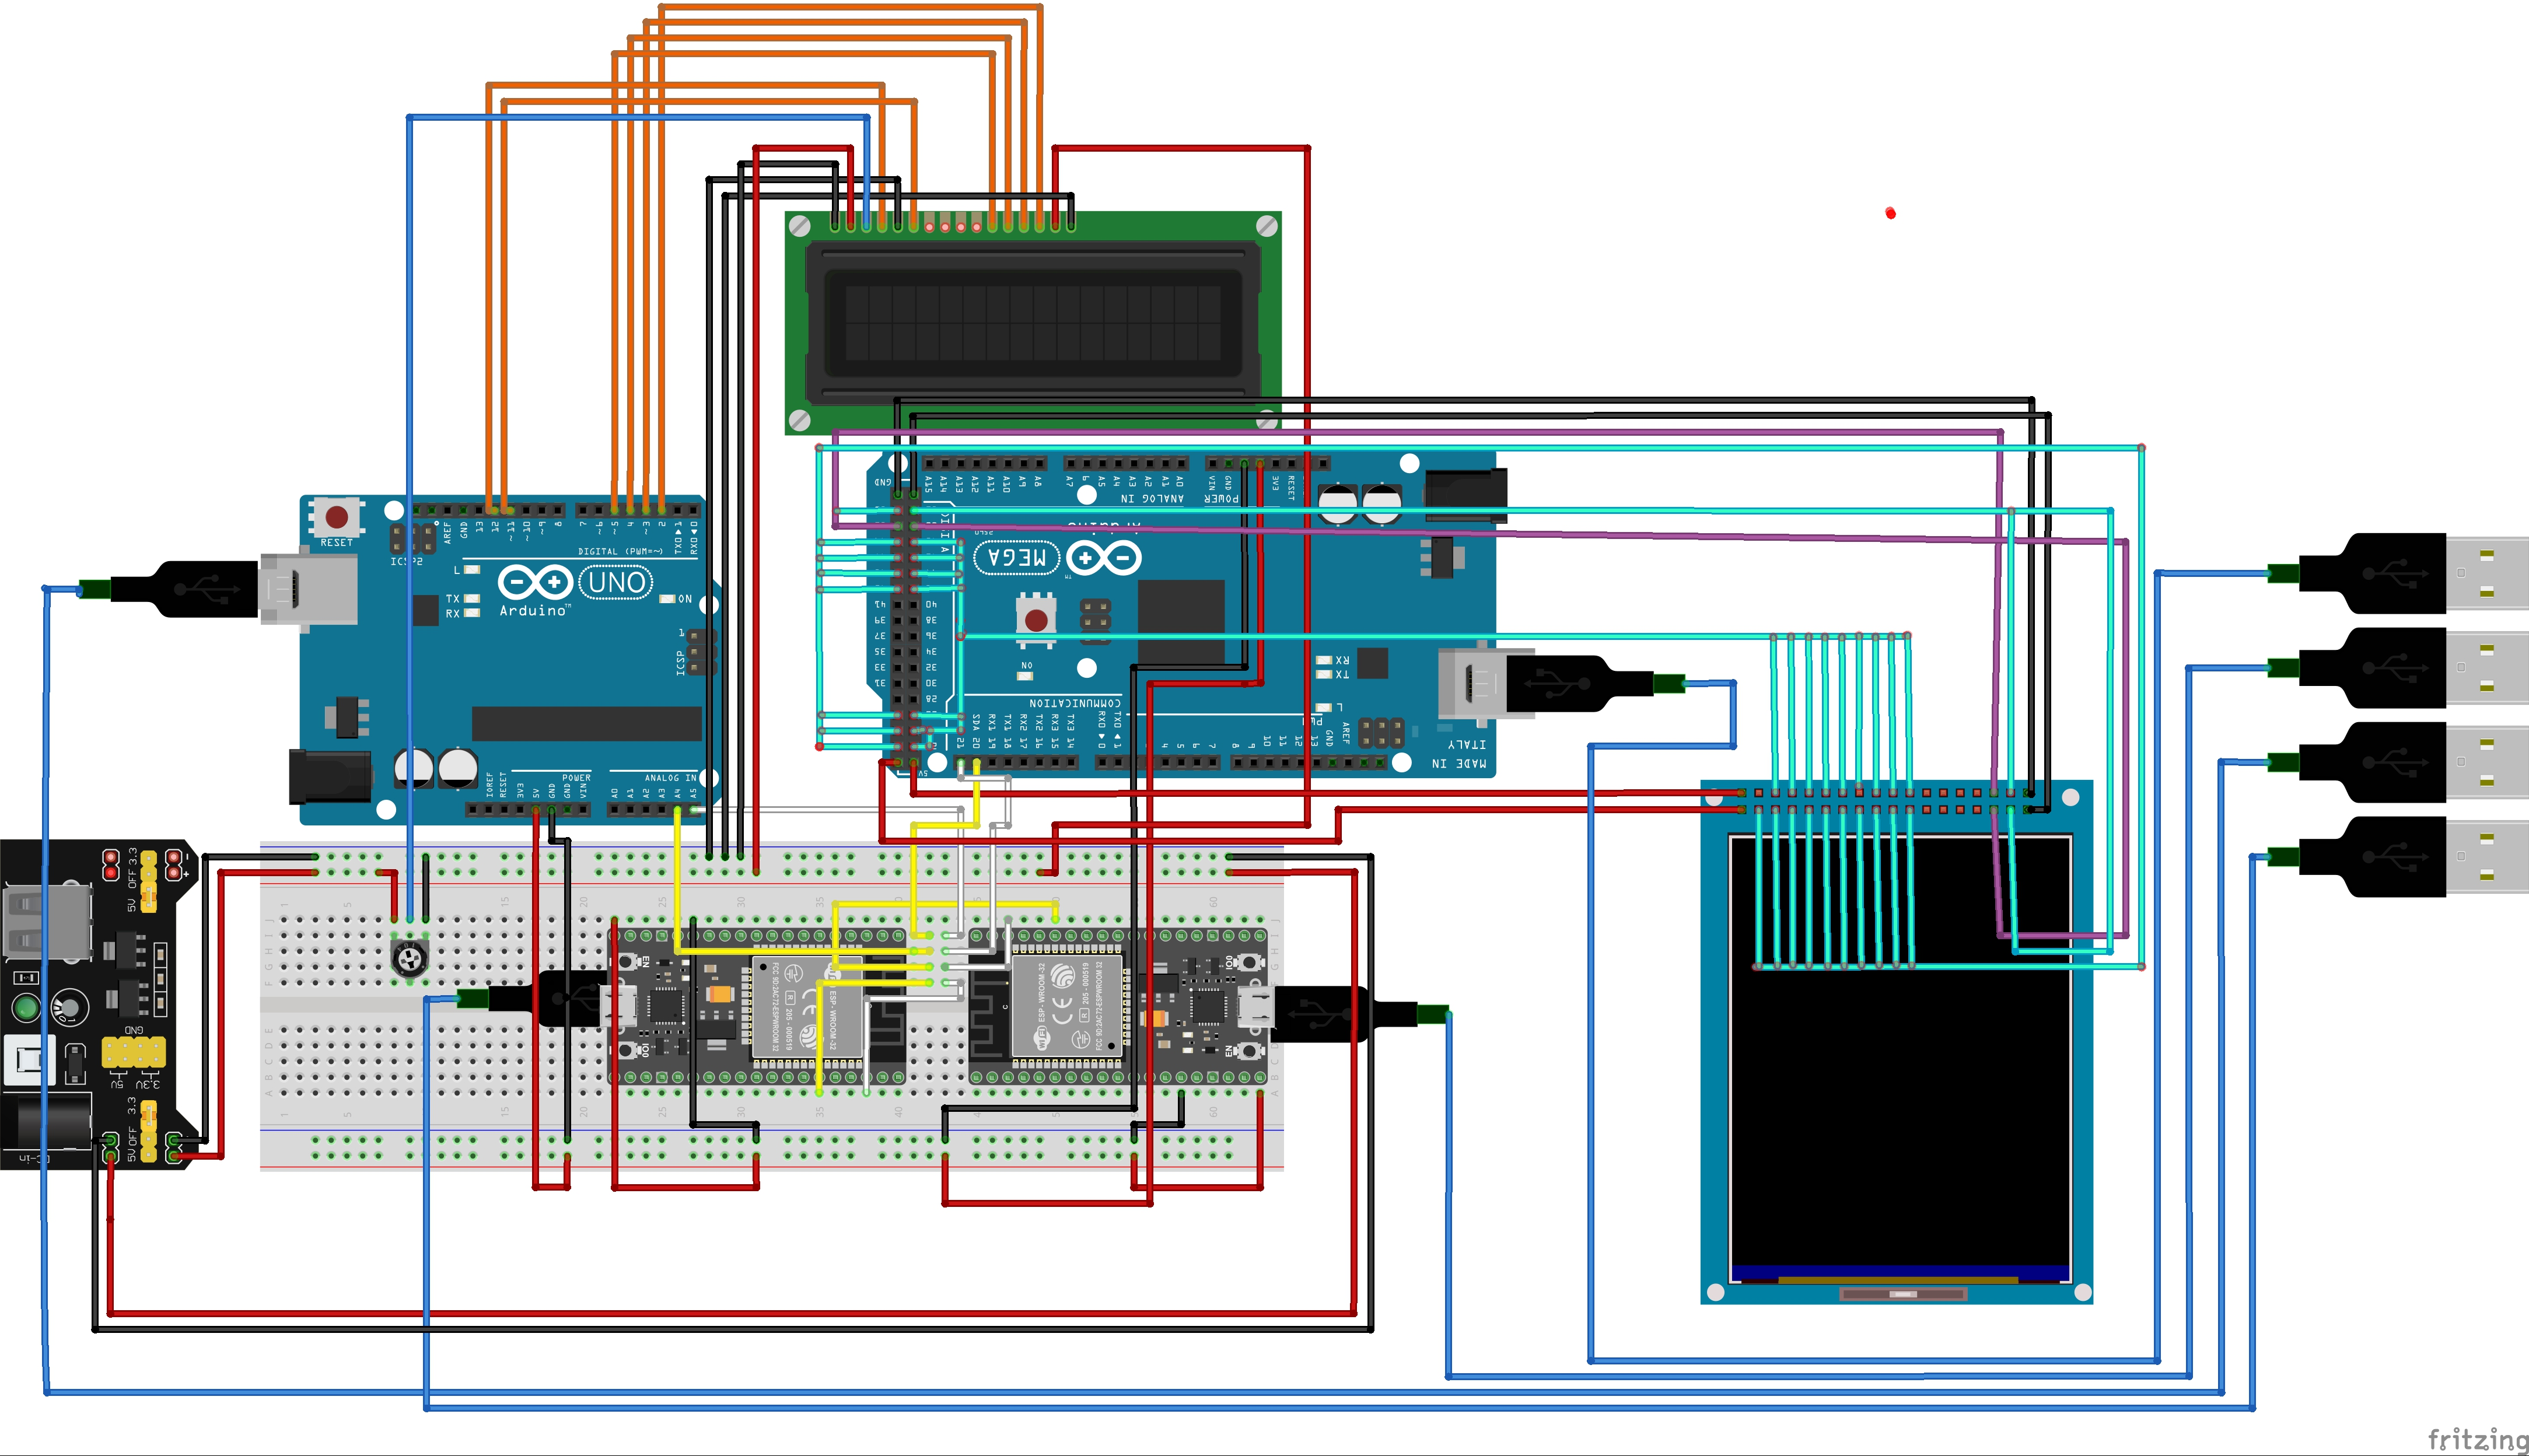
\includegraphics[width=0.8\textwidth]{/Users/renatorr/Downloads/coding/Github/SynthNet-Project-University/docs/README_FILES/circuitDiagram/circuit.jpg}
    \caption{Block diagram of the Synth Net system, showing the interconnected microcontrollers and their roles.}
    \label{fig:synthnet_diagram}
\end{figure}

As illustrated in Figure \ref{fig:synthnet_diagram}, the diagram showcases how the ESP32, Arduino Uno, and Arduino Mega are connected through the I2C bus and their respective functions in the system.


\documentclass{article}
\usepackage{graphicx}

\begin{document}

\section{Presentation Image}

\begin{figure}[h]
    \centering
    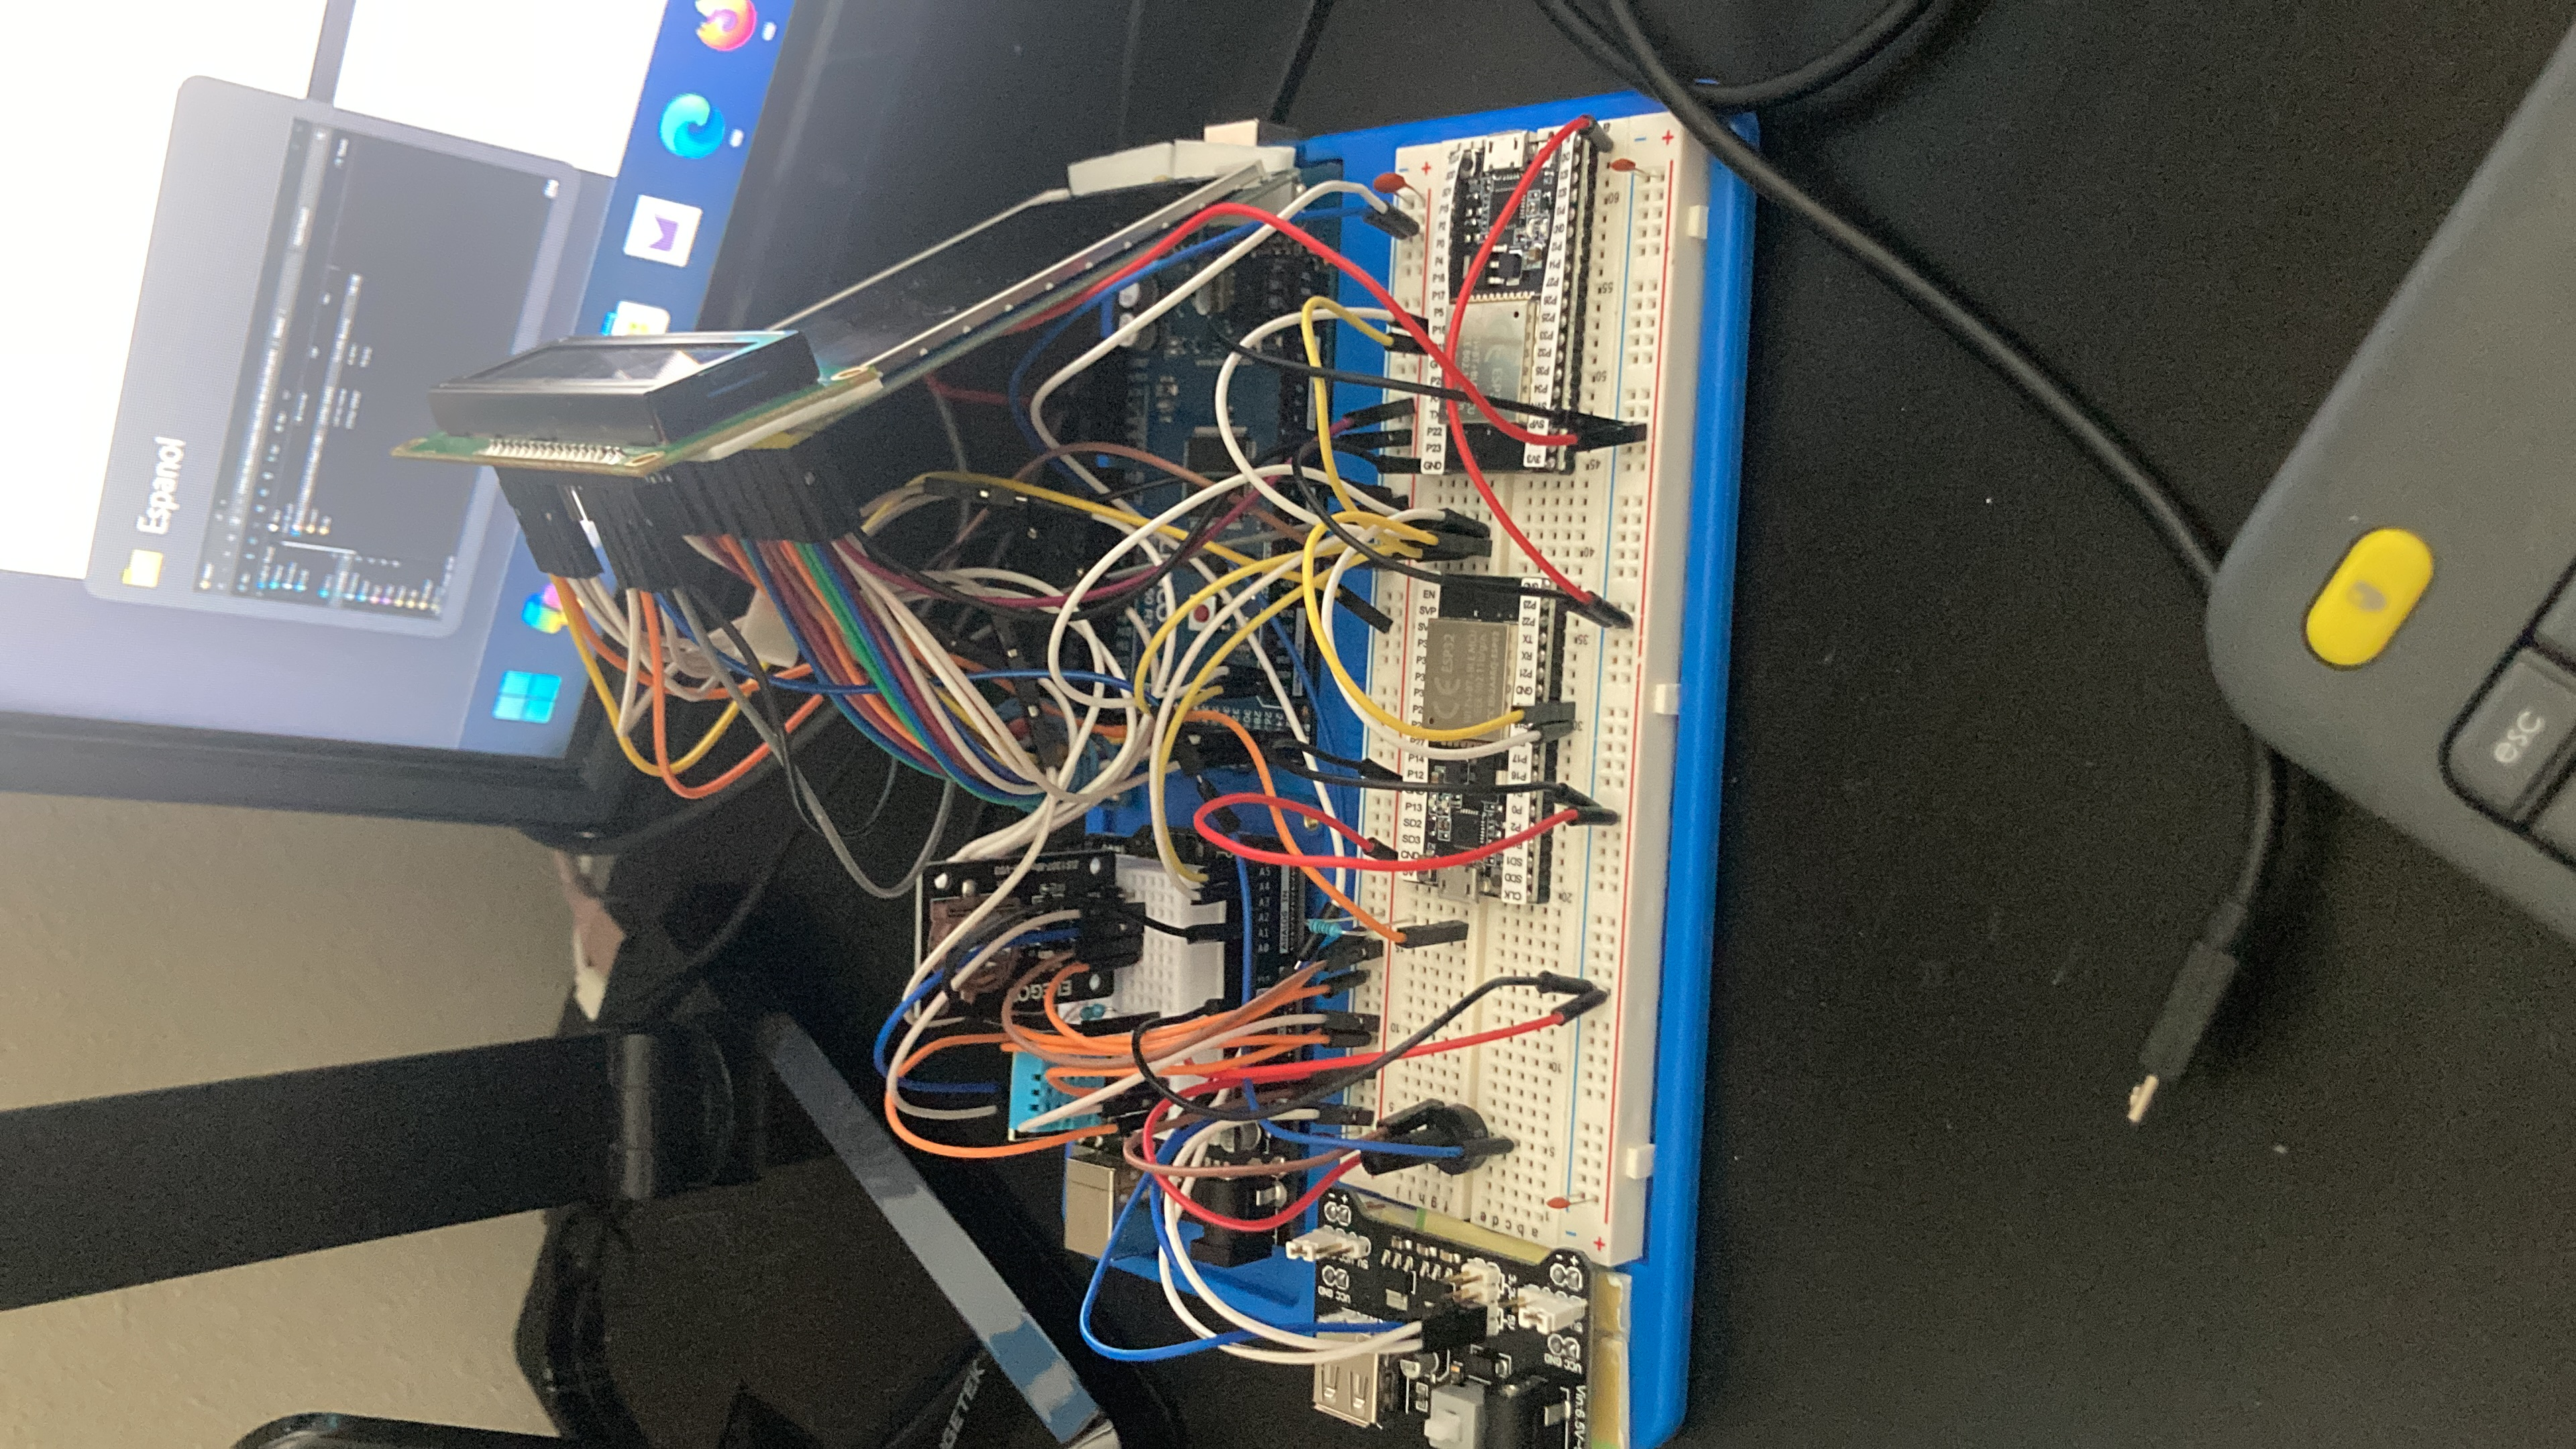
\includegraphics[width=0.8\textwidth]{docs/images/05726CB1-F2E2-489B-9CC1-331CCB7DC909.jpg}
    \caption{Presentation of Synth Net during the AI Industry Symposium and Career Mixer.}
    \label{fig:presentation_image}
\end{figure}

The image in Figure \ref{fig:presentation_image} captures the system presentation at the event, highlighting the key features of Synth Net.

\end{document}

\documentclass{article}
\usepackage{graphicx}

\begin{document}

\section{Oscilloscope Image}

\begin{figure}[h]
    \centering
    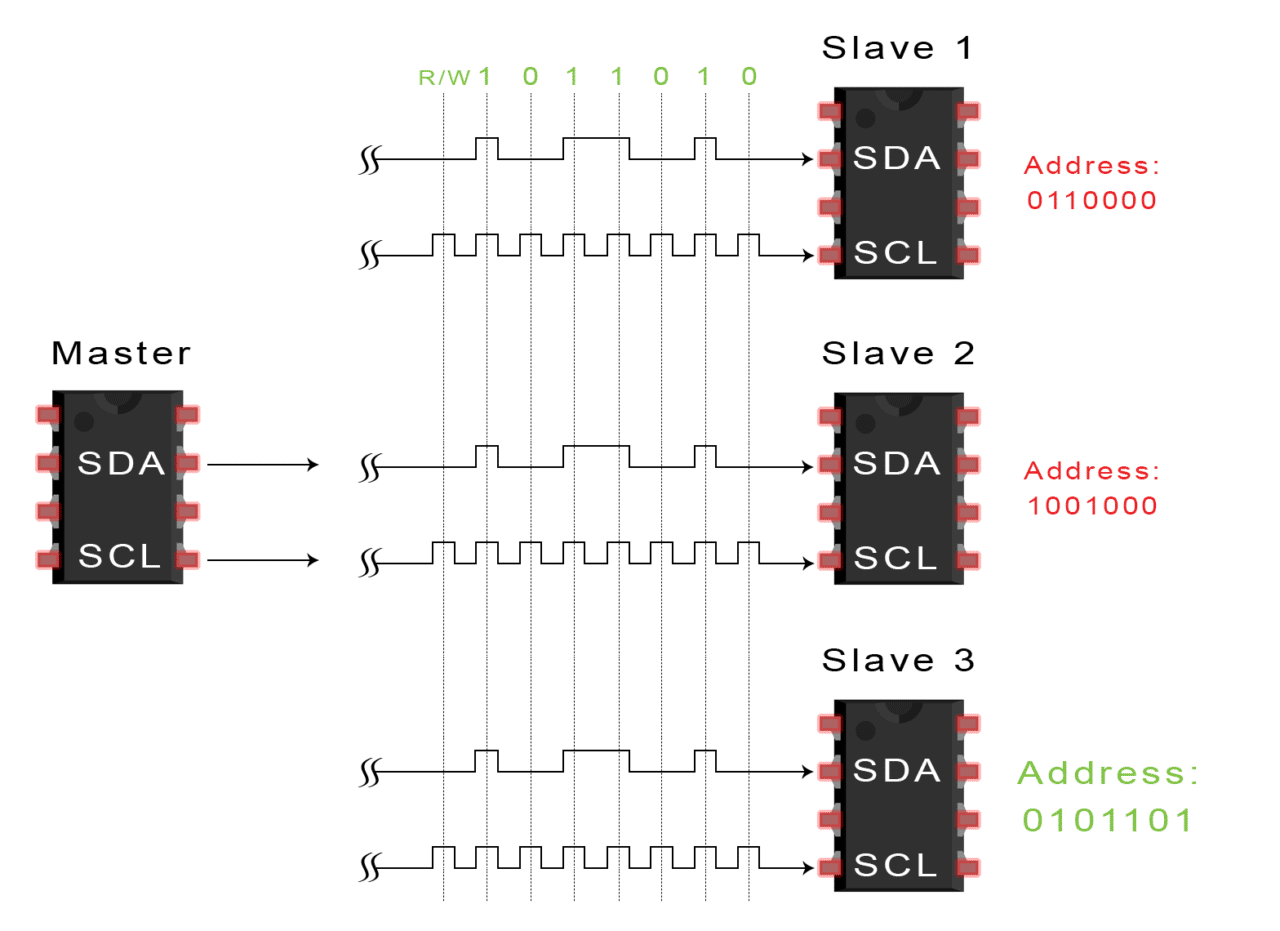
\includegraphics[width=0.8\textwidth]{/Users/renatorr/Downloads/coding/Github/SynthNet-Project-University/docs/images/diagrams.png}
    \caption{Oscilloscope reading of the I2C signal on the Synth Net system.}
    \label{fig:oscilloscope_image}
\end{figure}

Figure \ref{fig:oscilloscope_image} shows the oscilloscope capturing the I2C signal between the ESP32 and Arduino devices, demonstrating the data exchange process.

\end{document}

\end{document}

    
